%\documentclass[preprint]{sigproc}
\documentclass{acm_proc_article-sp}

% The following \documentclass options may be useful:
%
% 10pt          To set in 10-point type instead of 9-point.
% 11pt          To set in 11-point type instead of 9-point.
% authoryear    To obtain author/year citation style instead of numeric.

\setlength{\textfloatsep}{5pt}

\usepackage{flushend}
\usepackage{graphicx}
\usepackage{verbatim}
\usepackage{url}
\usepackage{alltt}
\renewcommand{\ttdefault}{txtt}

\usepackage{amsmath}
\usepackage{dsfont}
\usepackage{mathtools}
\everymath{\displaystyle}
\usepackage{xspace}

\newcommand{\CEU}{\textsc{C\'{e}u}\xspace}
\newcommand{\code}[1] {{\small{\texttt{#1}}}}
\newcommand{\DOFIN}{\code{do-finally}\xspace}
\newcommand{\FIN}{\code{finally}\xspace}

\newcommand{\ST}{\1\xrightarrow[~n~]{}\1}
\newcommand{\BT}{\xRightarrow[(i,E)]{}}
\newcommand{\LL}{\langle}
\newcommand{\RR}{\rangle}
\newcommand{\DS}{\displaystyle}
\newcommand{\rr}[1] {{\textbf{\scriptsize{#1}}}}


\newcommand{\1}{\;}
\newcommand{\2}{\;\;}
\newcommand{\3}{\;\;\;}
\newcommand{\5}{\;\;\;\;\;}
\newcommand{\ten}{\5\5}
\newcommand{\twenty}{\ten\ten}

\newenvironment{itemize*}%
  {\begin{itemize}%
    \setlength{\itemsep}{0pt}%
    \setlength{\parskip}{0pt}}%
  {\end{itemize}}

\usepackage{enumitem}
\setlist{nolistsep}

\usepackage{color}
\definecolor{light}{gray}{0.87}
\definecolor{dark}{gray}{0.30}
%\definecolor{light}{rgb}{.90,.90,.90}
\definecolor{darkgreen}{rgb}{0,.50,0}
\definecolor{darkblue}{rgb}{0,0,.50}
\definecolor{darkred}{rgb}{.50,0,0}
\definecolor{darkpur}{rgb}{.50,0,.50}

\usepackage{listings}
%\usepackage{textcomp}
\lstset{
%columns=fullflexible,
%basicstyle=\ttfamily,
escapeinside={||},
mathescape=true,
    language=C, % choose the language of the code
    basicstyle=\fontfamily{pcr}\selectfont\scriptsize\color{black},
    keywordstyle=\color{black}\bfseries, % style for keywords
    numbers=none, % where to put the line-numbers
    numberstyle=\tiny, % the size of the fonts that are used for the line-numbers
    backgroundcolor=\color{light},
    showspaces=false, % show spaces adding particular underscores
    showstringspaces=false, % underline spaces within strings
    showtabs=false, % show tabs within strings adding particular underscores
    %frame=single, % adds a frame around the code
    tabsize=2, % sets default tabsize to 2 spaces
    %rulesepcolor=\color{gray}
    captionpos=t, % sets the caption-position to bottom
    breaklines=false, % sets automatic line breaking
    %breakatwhitespace=false,
    numbersep=2em,
    emph={par,or,hor,do,end,loop,await,emit,input,event,call,with,command,%
          var,and,then,else,C,return,pure,deterministic,nohold,finalize,%
          class, every, FOREVER, this, spawn, in, pool, watching,
          each, abort, when, signal, PROC, CHAN, SIGNAL, PAR},
    emphstyle={\bfseries},
    commentstyle=\color{dark}\scriptsize,
    %xleftmargin=20pt,
    %xrightmargin=20pt,
    framesep=20pt,
    %upquote=true,
    %aboveskip={1.5\baselineskip},
}

\begin{document}
\sloppy

\title {
    %Imperative and Synchronous Abstractions for Reactive Applications
    %Structured Programming with Reactive Abstractions
    Structured Reactive Programming with C\'eu
}
%\subtitle{Accepted paper in REM'13 (preprint version)}

\numberofauthors{1}
\author{
    \alignauthor
    Francisco Sant'Anna \hspace{1cm} Roberto Ierusalimschy  \hspace{1cm} Noemi Rodriguez  \\
    \affaddr{Departamento de Inform\'atica --- PUC-Rio, Brasil} \\
    \email{\{fsantanna,roberto,noemi\}@inf.puc-rio.br}
}

\maketitle

\begin{abstract}
Through the language \CEU, we promote structured reactive programming as an 
extension to classical structured programming that also interacts continuously 
with the environment.
%
We revive the synchronous and imperative programming style of Esterel and aim 
to expand its limits from the strict embedded domain with the new abstraction 
mechanism of \emph{organisms}.

Organisms extend objects to react independently to the environment with an 
execution body that composes multiple lines of execution.
%
Compositions bring structured reasoning to concurrency and can better describe 
state machines typical of reactive applications.
%
Organisms are subject to lexical scope and automatic memory management similar 
to locals in a stack.
We show that this model does not require garbage collection or a \code{free} 
primitive in the language, eliminating memory leaks by design.
\end{abstract}

%\category{CR-number}{subcategory}{third-level}
%\category{D.3.1}{Programming Languages}{Formal Definitions and Theory}
%\category{D.3}{Programming Languages}{General}
\category{D.3.3}{Programming Languages}{Language Constructs and Features}

\terms{Design, Languages}

\keywords{Concurrency, Determinism, Esterel, Imperative, Structured 
Programming, Synchronous, Reactivity}

\section{Introduction}
\label{sec.intro}

Reactive applications interact continuously and in real time with external 
stimuli from the environment~\cite{statecharts.reactive,rp.synchronous}.
They represent a wide range of software areas and platforms: from games in 
powerful desktops, ``apps'' in capable smart phones, to the emerging internet 
of things in constrained embedded systems.

Research on special-purpose reactive languages dates back to the early 80's 
with the co-development of two complementary 
styles~\cite{rp.twelve,rp.hypothesis}:
%
The imperative style of Esterel~\cite{esterel.ieee91} organizes programs with 
structured control flow primitives, such as sequences, repetitions, and 
parallelism.
%
The dataflow style of Lustre~\cite{lustre.ieee91} represents programs as graphs 
of values, in which a change to a node updates its dependencies automatically.

In recent years, Functional Reactive Programming~\cite{frp.principles} 
modernized the dataflow style and became mainstream, deriving a number of 
languages and libraries, such as Flapjax~\cite{frp.flapjax}, Rx (from 
Microsoft), React (from Facebook), and Elm~\cite{frp.elm}.
%
In contrast, the imperative style of Esterel did not follow this trend and is 
now confined to the domain of real-time embedded control systems.
% such as flight control on avionics and anti-collision equipment on automobiles.

As a matter of fact, imperative reactivity is now often associated to the 
\emph{observer pattern}, typical in object oriented systems, because it heavily 
relies on side effects~\cite{rp.deprecating,rp.rescala}.
%
However, short-lived callbacks (i.e., the observers) eliminate any vestige of 
structured programming, such as support for long-lasting loops and automatic 
variables~\cite{sync_async.cooperative}, which are elementary capabilities of 
imperative languages.
%
In this sense, callbacks actually disrupt imperative reactivity, becoming ``our 
generation's \code{goto}''~\cite{dij.goto,rp.goto,elm.goto}.

In this work, we revive the imperative style of Esterel, which we now refer as 
\emph{Structured Reactive Programming (SRP)}.
%
SRP extends the classical hierarchical control constructs of \emph{Structured 
Programming (SP)} (i.e., concatenation, selection, and 
repetition~\cite{dij.notes}) to support continuous interaction with the 
environment.
%
In practical terms, SRP provides two extensions to SP:
an ``\code{await <event>}'' statement that suspends a line of execution until 
the referred event occurs, keeping all context alive;
and parallel constructs that compose multiple lines of execution and make them 
concurrent.
%
The \code{await} statement represents the imperative and reactive nature of 
SRP, recovering sequential execution lost with the observer pattern.
Parallel compositions%
\footnote{
We use the term \emph{parallel composition} as a synonym for \emph{side-by-side 
lexical composition}, which does not imply many-core parallel execution.
}
allow for multiple \code{await} statements to coexist, which is necessary to 
handle concurrent events, common in reactive applications.

We advocate SRP through the Esterel-based language \CEU~\cite{ceu.sensys13}, a 
contemporary outlook of imperative reactivity that aims to expand it from the 
rigid embedded domain.
%
%\CEU is based on Esterel and relies on a similar synchronous and deterministic 
%execution model that simplifies the reasoning about concurrency aspects.
%
We believe that the rigorous semantics of Esterel, which focus on static safety 
guarantees, is not suitable for other reactive application domains, such as 
GUIs, games, and distributed systems.
%
For instance, the lack of abstractions with dynamic lifetime makes difficult to 
deal with virtual resources such as graphical widgets, game units, and network 
sessions.

Our main contribution is a new abstraction mechanism for \CEU, the 
\emph{organisms}, that encapsulate parallel compositions with an object-like 
interface.
% that other parts of the program can manipulate.
%
In brief, organisms are to SRP like procedures are to SP, i.e., one can 
abstract a portion of code with a name and manipulate (call) that name from 
multiple places.
%
There are, however, additional challenges that apply to organisms:
%
\begin{itemize}
\item Organisms are themselves alive, acting as subprograms with continuous 
data and control state.
\item Organisms are part of a concurrent program that can manipulate and affect 
their data and execution state.
\item Organisms can be dynamically allocated, requiring a memory management 
model that must also apply to embedded systems.
\end{itemize}

The rest of the paper is organized as follows:
%Section~\ref{sec.models} justifies the synchronous concurrency model as better 
%choice for SRP.
Section~\ref{sec.ceu} presents SRP through \CEU, with its underlying 
synchronous concurrency model and powerful parallel compositions.
Section~\ref{sec.orgs} presents the organisms abstraction, which provides 
static and dynamic instances of subprograms with lexical scope and automatic 
memory management.
%Section~\ref{sec.demo} demonstrates a complete video game for Android 
%implemented in \CEU.
Section~\ref{sec.related} discusses related work.
Section~\ref{sec.conclusion} concludes the paper and makes final remarks.

\section{SRP with C\'eu}
\label{sec.ceu}

\CEU is a concurrent language, in which its lines of execution, known as 
\emph{trails}, react all together in synchronous steps and continuously to 
external stimuli.
%
Figure~\ref{lst.syntax} shows a compact reference of \CEU.

The introductory example of Figure~\ref{lst.intro} starts two trails with the 
\code{par} construct: the first (lines 4-8) increments variable \code{v} on 
every second and prints its value on screen; the second (lines 10-13) resets 
\code{v} on every external request to \code{RESET}.
%
%The input event \code{RESET} (line 1) represents the interface of the program 
%with external requests.
%The loop in the first trail (lines 4-8) continuously waits for 1 second, 
%increments variable \code{v}, and prints its current value.
%The loop in the second trail (lines 10-13) resets \code{v} on every occurrence 
%of \code{RESET}.
%
Programs in \CEU can access $C$ libraries of the underlying platform by 
prefixing symbols with an underscore (e.g., \code{\_printf(<...>)}).

\begin{figure}[t]
\begin{lstlisting}%[backgroundcolor=\color{white}]

// DECLARATIONS
input <type> <id>;        // external event
event <type> <id>;        // internal event
var   <type> <id>;        // variable

// EVENT HANDLING
await <id>;               // awaits event
emit  <id> => <exp>;      // emits  event

// COMPOUND STATEMENTS
<...> ; <...> ;           // sequence
if <...> then <...>       // conditional
         else <...> end
loop do <...> end         // repetition
    break                 //   (escape repetition)

// PARALLEL COMPOSITIONS
par/and do <...>          // rejoins on both sides
      with <...> end
par/or do  <...>          // rejoins on any side
      with <...> end
par do <...>              // never rejoins
  with <...> end

// C INTEGRATION
_f();                   // C call (prefix `_')
finalize <...>          // finalization
    with <...> end

// ORGANISMS
class <T> with
    <interface>
do
    <body>
end
\end{lstlisting}
%\rule{8.5cm}{0.37pt}
\caption{ Syntax of \CEU.
\label{lst.syntax}
}
\end{figure}

%%%%%%%%%%%%%%%%%%%%%%%%%%%%%%%%%%%%%%%%%%%%%%%%%%%%%%%%%%%%%%%%%%%%%%%%%%%%%%%
\subsection{Synchronous concurrency}
%%%%%%%%%%%%%%%%%%%%%%%%%%%%%%%%%%%%%%%%%%%%%%%%%%%%%%%%%%%%%%%%%%%%%%%%%%%%%%%

In the synchronous execution model of \CEU, a program must react completely to 
an occurring event before handling the next.
%
A reaction represents a logical instant in which all trails awaiting the 
occurring event awake and execute, one after the other, until they await again 
or terminate.
%
During a reaction, the environment is invariant and does not interrupt the 
running trails%
\footnote{
The actual implementation enqueues incoming input events to process them in 
further reactions.
}.
If multiple trails react to the same event, the scheduler employs lexical order 
to preserve determinism, i.e., the trail that appears first in the source code 
executes first.
%
To avoid infinite execution for reactions, \CEU ensures that all loops have 
\code{await} statements on their bodies~\cite{ceu.sensys13}.

As a result of synchronous execution, all operations to variable \code{v} in 
Figure~\ref{lst.intro} are atomic because reactions to \code{1s} and 
\code{RESET} can never interrupt each other.
%
In contrast, in asynchronous models with nondeterministic scheduling, the 
occurrence of \code{RESET} could preempt the first trail during an increment to 
\code{v} (line 6) and reset it (line 12) before printing it (line 7), 
characterizing a race condition on the variable.
%
The example illustrates the (arguably simpler) reasoning about concurrency 
aspects under the synchronous execution model.

\begin{figure}[t]
\begin{lstlisting}[numbers=left,xleftmargin=3em]
input void RESET;   // declares an external event
var int v = 0;
par do
    loop do         // 1st trail
        await 1s;
        v = v + 1;
        _printf("v = %d\n", v);
    end
with
    loop do         // 2nd trail
        await RESET;
        v = 0;
    end
end
\end{lstlisting}
\caption{ Introductory example in \CEU.
\label{lst.intro}
}
\end{figure}

%%%%%%%%%%%%%%%%%%%%%%%%%%%%%%%%%%%%%%%%%%%%%%%%%%%%%%%%%%%%%%%%%%%%%%%%%%%%%%%

The synchronous model also empowers SRP with an orthogonal abortion construct 
that simplifies the composition of activities%
\footnote{We use the term activity to generically refer to a language's unit of 
execution (e.g., \emph{thread}, \emph{actor}, \emph{trail}, etc.).}.
%
Orthogonal abortion is the ability to abort an activity from outside it, 
without affecting the overall consistency of the program (e.g., properly 
releasing global resources).
%
The example that follows shows the \code{par/or} construct of \CEU which 
composes trails and rejoin when either of them terminates, properly aborting 
the other:

\begin{lstlisting}
par/or do
    <body-trail-1>
with
    <body-trail-2>
end
<body-rejoin>
\end{lstlisting}

The \code{par/or} is regarded as orthogonal because the composed trails do not 
know when and how they are aborted (i.e., abortion is external to them).
%
%In the example, each trail has a set of local variables and an execution body 
%that lasts for an arbitrary time.
%After the \code{par/or} rejoins, a new set of local variables goes alive,
%reusing the space from the trails' locals going out of scope.

%\begin{figure}[t]
%\caption{ A \code{par/or} composes two concurrent trail and rejoins when one 
%terminates, aborting the other.
%\label{lst.abortion}
%}
%\end{figure}

Abortion in asynchronous languages is challenging~\cite{esterel.preemption} 
because the activity to be aborted might be on a inconsistent state (e.g., 
holding pending messages or locks).
%
This way, the language runtime needs to wait for the activity to be consistent 
before aborting it, resulting in two unsatisfactory semantics for a 
hypothetical \code{par/or}:
either wait to rejoin, making the program unresponsive to incoming events for 
an arbitrary time;
or rejoin immediately and let the activity complete termination in the 
background, which may cause race conditions with the subsequent code.
%which may confuse the programmer (which assumes both activities have 
%terminated), and also
%Immediate rejoin also leads to heap-based allocation (which is discouraged in 
%the context of embedded systems) because activities may coexist with the 
%subsequent code for some time.

In fact, asynchronous languages do not provide effective abortion:
\emph{Java}'s \code{Thread.stop} primitive has been officially 
deprecated~\cite{sync_async.threadsstop};
\emph{pthread}'s \code{pthread\_cancel} does not guarantee immediate 
cancellation~\cite{sync_async.pthreadsstop};
\emph{erlang}'s \code{exit} either enqueues a terminating message (which may 
take time), or unconditionally terminates the process (regardless of its 
state)~\cite{sync_async.erlangstop};
and \emph{CSP} only supports a composition operator that \emph{``terminates 
when \textbf{all} of the combined processes terminate''}~\cite{async.csp}.
%
As an alternative, asynchronous activities typically agree a on common protocol 
to abort each other (e.g., through shared state variables or message passing), 
increasing coupling among them with implementation details that are not 
directly related to the problem specification.

Synchronous languages, however, provide accurate control over the life cycle of 
concurrent activities because in between every reaction, the whole system is 
idle and consistent~\cite{esterel.preemption}.
%
In Section~\ref{sec.ceu.par} we show how \CEU deals with abortion of trails 
that use stateful resources from the environment, such as file and network 
handlers.

%\CEU provides the presented \code{par/or} construct, which is equivalent to 
%Esterel's \code{trap} abortion construct.
%
%In Section~\ref{sec.orgs} we highlight the importance of abortion for the 
%organisms abstraction.

%%%%%%%%%%%%%%%%%%%%%%%%%%%%%%%%%%%%%%%%%%%%%%%%%%%%%%%%%%%%%%%%%%%%%%%%%%%%%%%

%\subsection{The case for synchrony}

\subsection{Parallel compositions}
\label{sec.ceu.par}

\begin{comment}
- besides standard strucutred (loops, conditionals, sequences)
- add compositions
- await, sequence, vars
- parallel, patterns, ortoghonal
- finalize for C integration and keep orthogonality
    - no await inside it
- not really parallel (prev section)
\end{comment}

In terms of control structures, SRP basically extends SP with parallel 
compositions, allowing applications to handle multiple events concurrently.
%
\CEU provides three parallel constructs, which vary on how they rejoin:
a \code{par/and} rejoins when all trails in parallel terminate;
a \code{par/or} rejoins when any trail in parallel terminates;
a \code{par} never rejoins (even if all trails in parallel terminate).

The example that follows compares the \code{par/and} and \code{par/or} 
compositions side by side:

\begin{minipage}[t]{0.40\linewidth}
\begin{lstlisting}
// sampling pattern
loop do
    par/and do
        <...>
    with
        await 1s;
    end
end
\end{lstlisting}
\end{minipage}
%
\begin{minipage}[t]{0.40\linewidth}
\begin{lstlisting}
// timeout pattern
loop do
    par/or do
        <...>
    with
        await 1s;
    end
end
\end{lstlisting}
\end{minipage}

The code \code{<...>} represents a complex behavior with any degree of nested 
compositions.
%
In the \code{par/and} variation, the behavior repeats every second at minimum 
because both sides must terminate before re-executing the loop.
In the \code{par/or} variation, if the behavior does not terminate within 1 
second, it is restarted.
%
These SRP archetypes represent, respectively, the \emph{sampling} and 
\emph{timeout} patterns, which are typical of reactive applications.

%\begin{figure}[t]
%\rule{8.5cm}{0.37pt}
%\caption{ The \emph{sampling} and \emph{timeout} patterns using parallel 
%compositions.
%\label{lst.patts}
%}
%\end{figure}

\begin{figure}[t]
\begin{lstlisting}[numbers=left,xleftmargin=3em]
input void START, STOP, RETRANSMIT;
loop do
    await START;
    par/or do
        await STOP;
    with
        loop do
            par/or do
                await RETRANSMIT;
            with
                await <rand> s;
                par/and do
                    await 1min;
                with
                    <send-beacon-packet>
                end
            end
        end
    with
        <...> // the rest of the protocol
    end
end
\end{lstlisting}
%\rule{8.5cm}{0.37pt}
\caption{ Parallel compositions can describe complex state machines.
\label{lst.ctp}
}
\end{figure}

The code in Figure~\ref{lst.ctp} relies on hierarchical \code{par/or} and 
\code{par/and} compositions to describe the state machine of a protocol for 
sensor networks ported to \CEU~\cite{wsn.ctp,ceu.sensys13}.
%
The input events \code{START}, \code{STOP}, and \code{RETRANSMIT} (line 1) 
represent the external interface of the protocol with a client application.
%
The protocol enters the top-level loop and awaits the starting event (line 3).
Once the client application makes a start request, the protocol starts three 
other trails:
one to await the stopping event (line 5);
one to periodically transmit a status packet (lines 7-18);
and one with the remaining functionality of the protocol (collapsed in line 
20).
%
As compositions can be nested, the periodic transmission is another loop that 
starts two other trails (lines 8-17):
one to handle an immediate retransmission request (line 9);
and one to await a small random amount of time and transmit the status packet 
(lines 11-16).
%
The transmission (collapsed in line 15) is enclosed with a \code{par/and} that 
takes at least one minute before looping to avoid flooding the network.
%
At any time, the client may request a retransmission (line 9), which terminates 
the \code{par/or} (line 8), aborts the ongoing transmission (line 15, if not 
idle), and restarts the loop (line 7).
%
Also, the client may request to stop the whole protocol at any time (line 5), 
which terminates the outermost \code{par/or} and aborts the transmission and 
all composed trails.
In this case, the top-level loop restarts and waits for the next request to 
start the protocol (line 3), ignoring all other requests as specified.

The example shows how parallel compositions can describe complex state machines 
in a structured way, eliminating the use of global state variables for this 
purpose~\cite{ceu.sensys13}.

\subsubsection{Finalization}

\begin{figure}[t]
\begin{minipage}[t]{0.45\linewidth}
\begin{lstlisting}
var _message_t buffer;
<fill-buffer-info>
_send_enqueue(&buffer);
await SEND_ACK;
\end{lstlisting}
\end{minipage}
%
\begin{minipage}[t]{0.50\linewidth}
\begin{lstlisting}
var _message_t buffer;
<fill-buffer-info>
finalize
    _send_enqueue(&buffer)
with
    _send_dequeue(&buffer);
end
await SEND_ACK;
\end{lstlisting}
\end{minipage}
%\rule{8.5cm}{0.37pt}
\caption{ Finalization clauses safely release low-level resources.
\label{lst.fin}
}
\end{figure}

\begin{figure*}[t]
\begin{minipage}[t]{0.28\linewidth}
\begin{lstlisting}
par/or do
    loop do
        await 600ms;
        _toggle(11);
    end
with
    loop do
        await 1s;
        _toggle(12);
    end
with
    await 1min;
end


















/* CODE-1: original blinking */
\end{lstlisting}
\end{minipage}
%
\begin{minipage}[t]{0.32\linewidth}
\begin{lstlisting}[numbers=left,xleftmargin=3.5em]
class Blink with
    var int pin;
    var int dt;
do
    loop do
        await (this.dt)ms;
        _toggle(this.pin);
    end
end

do
    var Blink b1 with
        this.pin = 11;
        this.dt  = 600;
    end;

    var Blink b2 with
        this.pin = 12;
        this.dt  = 1000;
    end;

    await 1min;
end








/* CODE-2: blinking organisms */
\end{lstlisting}
\end{minipage}
%
\begin{minipage}[t]{0.34\linewidth}
\begin{lstlisting}[numbers=left,xleftmargin=3.5em]
struct _Blink with
    var int pin;
    var int dt;
end;

do
    var _Blink b1, b2;

    par/or do
        // body of b1
        b1.pin = 11;
        b1.dt  = 600;
        loop do
            await (b1.dt)ms;
            _toggle(b1.pin);
        end
        await FOREVER;
    with
        // body of b2
        b2.pin = 12;
        b2.dt  = 1000;
        loop do
            await (b2.dt)ms;
            _toggle(b2.pin);
        end
        await FOREVER;
    with
        await 1min;
    end
end

/* CODE-3: organisms expansion */
\end{lstlisting}
\end{minipage}
%
%\rule{17.5cm}{0.37pt}
\caption{ Two blinking LEDs using organisms.
\label{lst.orgs}
}
\end{figure*}

\begin{comment}
\begin{figure}[t]
\begin{lstlisting}[numbers=left,xleftmargin=3em]
<...>
    par/or do
        await STOP;
    with
        <...>
            par/or do
                await RETRANSMIT;
            with
                <...>
            end
    end
\end{lstlisting}
%\rule{14cm}{0.37pt}
\caption{
\label{lst.ctp}
}
\end{figure}
\end{comment}

%Programs in \CEU can access $C$ libraries available in the underlying platform 
%by prefixing symbols with an underscore (e.g., \code{\_printf(<...>)}).
%
The \CEU compiler tracks the interaction of \code{par/or} compositions with 
local variables and stateful native $C$ functions (e.g., device drivers) to 
guarantee that trail abortion is always safe.

Consider the code on the left of Figure~\ref{lst.fin}, which expands the 
sending trail of Figure~\ref{lst.ctp} (line 15).
%
The \code{buffer} packet is a local variable whose pointer is passed to native 
function \code{\_send\_enqueue}.
The call enqueues the pointer in the radio driver, which holds it up to the 
occurrence of \code{SEND\_ACK} acknowledging the packet transmission.
%
In the meantime, the sending trail might be aborted from \code{STOP} or 
\code{RETRANSMIT} requests (lines 5 and 9 of Figure~\ref{lst.ctp}), making the 
packet buffer to go out of scope, and leading to a \emph{dangling pointer} in 
the radio driver.
%
\CEU refuses to compile programs like this and requires \emph{finalization} 
clauses to accompany stateful native calls~\cite{ceu.sensys13}.
The code on the right of Figure~\ref{lst.fin} properly dequeues the packet if
the block of \code{buffer} goes out of scope, i.e., the finalization clause 
after the \code{with} executes automatically on abortion.

Finalization clauses are fundamental to preserve the orthogonality of 
\code{par/or} compositions in SRP.

\section{Organisms: SRP Abstractions}
\label{sec.orgs}

Applications often need to replicate a behavior and rely on abstractions that 
the language provide.
%
In SP, the typical abstraction mechanism are procedures, which abstract
recurrent routines with meaningful names that can be invoked multiple times 
with different parameters.
%
However, procedures have a single entry point, and were not devised for 
continuous and concurrent input.
For instance, procedures cannot express parallel compositions as described in 
Section~\ref{sec.ceu.par}.
%
The prevailing imperative abstraction mechanism for reactive applications are 
objects used in conjunction with the observer pattern.
Even though objects abstract data with proper encapsulation, they cannot 
encapsulate control flow because methods have to return control as quickly as 
possible to keep the application responsive~\cite{TODO.games.patterns}.

\CEU abstracts data and control state into the single concept of organisms.
%Organisms provide an execution body with multiple lines of execution (control 
%state) as well as object-like interface (data state).
%
A class of organisms describes an interface and a single execution body.
The interface exposes public variables, methods, and also internal events.
The body can contain any valid code in \CEU, including parallel compositions.
When an organism is instantiated, its body starts to execute in parallel with 
the program.
Organism instantiation can be either static or dynamic.
% TODO: The syntax xxx

The example of Figure~\ref{lst.orgs} introduces static organisms through three 
code chunks:
%
\begin{itemize}
\item The leftmost code (\emph{CODE-1}) blinks two LEDs with different 
frequencies in parallel and terminates after 1 minute.
%
\item The code in the middle (\emph{CODE-2}) abstracts the blinking LEDs in an 
organism class and uses two instances to reproduce the same behavior of 
\emph{CODE-1}.
%
\item The rightmost code (\emph{CODE-3}) is the equivalent expansion of the 
organisms bodies, which should resemble the original \emph{CODE-1}.
\end{itemize}
%
In \emph{CODE-2}, the Blink class (lines 1-9) exposes the \code{pin} and 
\code{dt} properties, corresponding to the LED I/O pin and the blinking period, 
respectively.
The application then creates two instances, specifying those properties in the 
constructors (lines 12-15 and 17-20).
Inside constructors, the identifier \code{this} refers to the organism under 
instantiation.
The constructors also start the organisms bodies (lines 5-8) to run in parallel 
in the background, i.e., both instances are already running before the 
\code{await 1min} (line 22).

\emph{CODE-3} is semantically equivalent to \emph{CODE-2}, but with the 
organisms constructors and bodies expanded (lines 11-16 and 20-25).
The generated \code{par/or} makes the instances and the rest of the application 
(i.e., \code{await 1min}, in line 28) concurrent.
Note the \code{await FOREVER} statements (lines 17 and 26) to avoid the 
organisms bodies to terminate the \code{par/or}.
The \code{\_Blink} type (lines 1-4) corresponds to a simple datatype without an
execution body.
%
The actual implementation of \CEU does not expand the organisms bodies like in 
\emph{CODE-3}, instead, a class generates a single code for its body, which is 
shared by all instances (in the same way as objects share class methods).

The main distinction from organisms to standard objects is how they can react 
independently and directly to the environment, i.e., once instantiated they 
become alive and reactive (hence the name \emph{organisms}).
%
For instance, organisms need not be included in observer lists for events, or 
rely on the main program to feed their methods with input from the environment.
%
Even tough the organisms run independent from the main program, they are still 
subject to the disciplined synchronous model, which keeps the whole system 
deterministic, as the static expansion to \emph{CODE-3} suggests.
%
%\emph{CODE-3} shows that the equivalent expansion results in plain \CEU.

The memory model for organisms eliminates memory leaks, dangling pointers, and 
the need for garbage collection.
%
The model is similar to stack-living local variables of procedures, providing 
lexical scope and automatic bookkeeping of organisms.
We also restrict explicit manipulation of references to organisms to avoid 
unsafe access after they go out of scope, as we discuss in 
Section~\ref{sec.orgs.refs}.

Regarding lexical scope and automatic memory management, note that 
\emph{CODE-2} uses a \code{do-end} block (lines 11-23) that limits the scope of 
the organisms for 1 minute (line 22).
%
During that period, the organisms are accessible (through \code{b1} and 
\code{b2}) and reactive to the environment.
%
In the equivalent expansion of \emph{CODE-3}, the \code{par/or} (lines 9-29) 
aborts the organisms bodies after that period (line 28), just before they go 
out of scope (line 30).
%
In addition, the \code{par/or} termination properly triggers all active 
finalization clauses inside the organisms.
%
Lexical scope extends the idea of orthogonal abortion to organisms, as they are 
automatically aborted when going out of scope.

In addition to properties and methods, organisms also expose internal events 
which support \code{await} and \code{emit} operations.
%
In the example of Figure~\ref{lst.unit}, the class \code{Unit} (lines 1-16) 
defines the position property \code{pos} with default vaule \code{0} (line 2), 
and the event \code{move} which exposes requests to move the unit position 
(line 3).
%
The main program (lines 18-28) creates two units and requests them to move to 
position \code{500} with a interval of 1 second.
%
The body of the class initializes the current unit's destination position 
\code{dst} to the current position (line 5).
Then, the body enters in a continuous loop (lines 6-15) to handle \code{move} 
requests (line 8) while performing the actual moving operation (lines 10-13) in 
parallel.
The \code{par/or} restarts the loop on every \code{move} request, which updates 
the \code{dst} position.
%
The moving operation can be as complex as needed, for example, using another 
loop to apply physics over time.
The \code{await FOREVER} (line 13) halts the trail after the move completes.
%
An advantage of event handling over method calls is that they can be composed 
in the organism body to affect other ongoing operations.
In the example, the \code{await move} (line 8) aborts and restarts the moving 
operation, just like the timeout pattern of Section~\ref{sec.ceu.par}.

\begin{figure}[t]
\begin{lstlisting}[numbers=left,xleftmargin=3em]
class Unit with
    var   int pos = 0;
    event int move;
do
    var int dst = this.pos;
    loop do
        par/or do
            dst = await this.move;
        with
            if dst != pos then
                <code-to-move-pos-to-dst>
            end
            await FOREVER;
        end
    end
end

var Unit u1 with
    this.pos = 100;
end;

var Unit u2 with
    this.pos = 200;
end;

emit u1.move => 500;
await 1s;
emit u2.move => 500;
\end{lstlisting}
%\rule{8.5cm}{0.37pt}
\caption{ Organism manipulation through interface events.
\label{lst.unit}
}
\end{figure}

%\newpage
\subsection{Dynamic organisms}

Static embedded systems typically manipulate real sensors and actuators 
hardware with a one-to-one correspondence in software, i.e., a static (possibly 
complex) piece of software deals with a corresponding piece of hardware.
%
In contrast, more general reactive systems have to deal with resource 
virtualization, such as multiplexing protocols in a network, or simulating 
entire civilizations in a game.
%
Dynamic allocation for organisms extends the power of SRP to handle virtual 
resources in reactive applications.

\CEU supports dynamic instantiation of organisms through the \code{spawn} 
primitive.
The example that follows spawns a new instance of \code{Unit} on
every second and moves it to a random position:

\begin{lstlisting}
every 1s do
    var Unit* u = spawn Unit with
                      this.pos = _rand() % 500;
                  end;
    emit u:move => _rand() % 500;
end
\end{lstlisting}

The \code{spawn} allocates the new organism and returns a pointer to it, which 
can be later dereferenced with the operator \code{`:'} (analogous to 
\code{`->'} of \emph{C/C++}).

%\begin{figure}[t]
%\rule{8.5cm}{0.37pt}
%\caption{ Spawns and moves a new \code{Unit} every second.
%\label{lst.spawn}
%}
%\end{figure}

Dynamic instances also execute in parallel with the rest of the application, 
but have different lifetime and scoping rules:
%
A static instance has a unique identifier and a well-defined scope that holds 
its memory resources;
A dynamic instance outlives the scope that spawns it and is anonymous (but may 
have pointers to it, as in the previous example).

In accordance with the reactive and independent nature of organisms, \CEU 
supports that a dynamic instance control its own lifetime:
once its body terminates, a dynamic organism is automatically freed from 
memory.
%
The example that follows redefines the body of the \code{Unit} class of 
Figure~\ref{lst.unit} to terminate after 1 hour, imposing a maximum life span 
in which a unit can react to \code{move} requests.
After that, the body terminates and the organism is automatically freed:

%\begin{figure}[t]
\begin{lstlisting}
class Unit with
    <...>           // interface
do
    par/or do
        <...>       // moving trail
    with
        await 1h;
    end
end
\end{lstlisting}
%\rule{8.5cm}{0.37pt}
%\caption{ The \code{Unit} body terminates after 1 hour.
%\label{lst.free}
%}
%\end{figure}

The lack of scopes for dynamic organisms prevents orthogonal abortion, given 
that there is no way to externally abort the execution of dynamic instances.
%
To overcome this limitation, \CEU provides lexically scoped \emph{pools} as 
containers that hold dynamic organisms instances.
%
The example that follows declares the \code{units} pool that holds a maximum of 
10 instances (line 3):

%\begin{figure}[t]
\begin{lstlisting}[numbers=left,xleftmargin=3em]
input void CLICK;
do
    pool Unit[10] units;
    par/or do
        every 1s do
            spawn Unit in units with
                <...>   // constructor
            end;
        end
    with
        await CLICK;
    end
end
\end{lstlisting}
%\rule{8.5cm}{0.37pt}
%\caption{ Spawns and moves a new \code{Unit} every second.
%\label{lst.pool}
%}
%\end{figure}

A new unit is spawned in this pool on every second (note the \code{in units}, 
in line 6).
Once the application receives a \code{CLICK} (line 11), the \code{par/or} 
terminates, making the \code{units} pool to go out of scope and abort/free all 
units alive.

Pools with dimension (e.g., \code{pool Unit[10] units}), have static 
pre-allocation, resulting in efficient and deterministic organism 
instantiation.
This opens the possibility for dynamic behavior also in constrained embedded 
systems.
%
If a pool does not specify a dimension (e.g., \code{pool Unit[] units}), the 
instances go to the heap but are still subject to the pool scope.
%
If a \code{spawn} does not specify a pool, as in ``\code{spawn Unit;}'', the 
instances go to a predefined dimension-less pool in the top of the current 
class (and are subject to that pool scope).

Note that lexical scope support for both static and dynamic organisms eliminate 
garbage collection, \code{free} primitives, and memory leaks altogether.

\begin{comment}
Pools provide iterators to access pointers to all alive instances.
The example that follows iterates over the \code{units} pool and requests each 
unit to move to a random position:

%\begin{figure}[t]
\begin{lstlisting}
pool Unit[10] units;
<...>
loop (Unit*)u in units do
    emit u:move => _rand() % 500;
end
\end{lstlisting}
%\rule{8.5cm}{0.37pt}
%\caption{ Iterating over a pool.
%\label{lst.iter}
%}
%\end{figure}
\end{comment}

\subsection{Pointers and References}
\label{sec.orgs.refs}

As organisms react independently from the environment, it is often not 
necessary to hold pointers to organisms.
%
In fact, pointers can be dangerous because they may last longer than the 
organisms they refer:

\begin{lstlisting}
var Unit* u = <...>;
u:pos = 0;              // this access is safe
await 2h;
emit u:move => 100;     // this access is unsafe
\end{lstlisting}

The example first acquires a pointer \code{u} to \code{Unit} somehow.
Then, it dereferences the pointer in two occasions:
in the same reaction, just after acquiring the reference;
and in another reaction, after \emph{2h}, when the pointed organism may have 
already terminated and being freed.

\CEU enforces all pointer accesses across reactions to use the \code{watching} 
construct which supervises organism termination:

\begin{minipage}[t]{0.48\linewidth}
\begin{lstlisting}
var Unit* u = <...>;
u:pos = 0;
watching u do
    await 2h;
    emit u:move => 100;
end
\end{lstlisting}
\end{minipage}
%
\begin{minipage}[t]{0.48\linewidth}
\begin{lstlisting}
var Unit* u = ...;
u:pos = 0;
par/or do
    await u:__killed;
with
    await 2h
    emit u:move => 100;
end
\end{lstlisting}
\end{minipage}

The whole \code{watching} construct aborts whenever the referred organism 
terminates, eliminating possible dangling pointers in the program.
%
The code in the right shows the equivalent expansion of the \code{wacthing} 
construct to a \code{par/or} that awaits the special event \code{\_\_killed}.

\begin{comment}

% TODO: weak vs strong references

\CEU distinguishes weak references (pointers) from strong references.
A strong reference
(references, for short).

class Unit with
    <...>
    var Weapon& weapon;
do
    <...>
    emit weapon.fire;
end
var Weapon w;
var Unit u with
    this.weapon = w;
end;

scopes
    - solve the problem of lapsed listener

- interaction
    - events
    - data
    - exemplo do Ship?

- procedure equivalence
    do T with
        ...
    end

    do
        var T t;
        await t.ok;
    end

    class T with
        event void ok;
    do
    end

- pools
- iterators
- weak/strong references (also for static)

- CONCL.
- ORGS relies on par/or for bodies and track refs
\end{comment}

%\section{Applications}
%\subsection{WSN ring}
%\subsection{Game}

\section{Related work}
\label{sec.related}

Esterel provides a module abstraction through the \code{run} command, which 
syntactically replaces the command by the referred module 
body~\cite{esterel.primer}.
%
Similarly, ESPranto~\cite{espranto} extends Esterel with a macro-based 
abstraction mechanism that enables the creation of domain specific languages.
%
However, macros expand at compile-time, being impossible to describe dynamic 
instantiation.
Furthermore, each use of a macro results in code replication, having a negative 
impact on code size.

Simula is a simulation language that introduced the concepts of objects and 
coroutines~\cite{simula}.
%
The syntactic structure of classes in Simula is very similar to \CEU, exposing 
an interface that encapsulates an execution body.
%
However, the underlying execution models are fundamentally distinct:
\CEU employs a reactive scheduler to resume trails based on external stimuli, 
while Simula relies on cooperation between processes (i.e., \code{detach} and 
\code{resume} calls, at the lowest level).
%
Simula has no notion of compositions and each process has a single line of 
execution.
In particular, the lack of a \code{par/or} precludes orthogonal abortion and 
many derived \CEU features, such as lexically scoped organisms, finalization, 
and reference watching.
%
Without scopes, Simula objects and processes have to live on the heap and rely 
on garbage collection.
As far as we know, Simula processes cannot be terminated explicitly from other 
processes.
%
%Finally, the conjunction of compositions with the synchronous model of \CEU 
%enables a XXX of static analysis, such as concurrent accesses to 
%variables~\cite{ceu.sensys13}.

Even though Simula and Esterel are considerably old languages, their core ideas 
that apply to \CEU have not evolved significantly, namely objects with an 
execution body, compositions with orthogonal abortion, and the reactive 
synchronous model.

\begin{comment}
- asynchronous langs
- Esterel + descendants
- CRP
- simula
- FRP

interactive  vs reactive
asynchronous vs synchronous
dataflow vs control
dynamic vs static

imperative
    - sequential (eliminates state machines)
    - better resource control
    - less abstract

dataflow

exemplo data melhor vs control melhor

The synchronous concurrency model...

We show composibility, sequential, imperative
safety
Then, we extend synchronous reactive programming with dynamic

control vs data reactivity
\end{comment}

\section{Conclusion}
\label{sec.conclusion}

\CEU provides comprehensive support for structured reactive programming, 
extending classical structure programming with continuous interaction with
external stimuli.

\CEU introduces organisms which reconcile data and control state in a single 
abstraction.
%
In contrast with objects, organisms have an execution body that can react 
independently to stimuli from the environment.
%
Both static and dynamic instances of organisms are subject to lexical scope 
with automatic memory management, which eliminates memory leaks and the need 
for a garbage collector.

\CEU is suitable for wide range of reactive applications and platforms.
%
We have been using it in constrained platforms for sensor networks (e.g., 16MHz 
CPU with 4Kb of RAM) as well as in full-fledged tablets for games and graphical 
applications.

%care with embedded systems
%- pool
%- GC

%- examples w/o watching

%- games

%- wsn

\begin{comment}

===============================================================================

In computing, reactive programming is a programming paradigm oriented around data flows and the propagation of change. This means that it should be possible to express static or dynamic data flows with ease in the programming languages used, and that the underlying execution model will automatically propagate changes through the data flow.

For example, in an imperative programming setting, a := b + c would mean that a is being assigned the result of b + c in the instant the expression is evaluated. Later, the values of b and c can be changed with no effect on the value of a.

In reactive programming, the value of a would be automatically updated based on 
the new values.

===============================================================================

There seems to be a lot of confusion about Reactive Programming. What is it? Who created it?

The earliest reference I could find was written by Gérard Berry (one of the creators of the Esterel dataflow language) in his 1989 paper, “Real time programming: Special purpose or general purpose languages.” I emailed him to see if he knew of an earlier use. Mr. Berry pointed me to the 1985 paper, “On the development of reactive systems” by David Harel and Amir Pnueli. After contacting Professor Harel, he confirmed that they where the originators of the term.

So it would seem that Reactive Programming is at least 30 years old.

Harel and Pnueli’s paper discussed designing reactive systems in general, software or hardware. Their definition was…

    “Reactive systems… are repeatedly prompted by the outside world and their role is to continuously respond to external inputs.”

    D. Harel and A. Pnuli, “On the Development of Reactive Systems” (1985)

Mr. Berry’s paper focused on the software aspects of Reactive Programming…

    “It is convenient to distinguish roughly between three kinds of computer programs. Transformational programs compute results from a given set of inputs; typical examples are compilers or numerical computation programs. Interactive programs interact at their own speed with users or with other programs; from a user point of view a time-sharing system is interactive. Reactive programs also maintain a continuous interaction with their environment, but at a speed which is determined by the environment, not by the program itself. Interactive programs work at their own pace and mostly deal with communications, while reactive programs only work in response to external demands and mostly deal with accurate interrupt handling.

    Real-time programs are usually reactive. However, there are reactive program that are not usually considered as being real-time, such as protocols, system drivers or man-machine interface handlers. All reactive programs require a common programming style.

    Complex applications usually require establishing cooperation between the three kinds of programs. For example, a programmer uses a man-machine interface involving menus, scroll bars and other reactive devices. The reactive interface permits him to tell the interactive operating systems to start transformational computations such as program compilations.”

    Berry, Gérard. “Real time programming: Special purpose or general purpose languages.” (1989)

From the preceding quotes we can say that reactive programs…

    Activate in response to external demands
    Mostly deal with handling parallelism
    Operate at the rate of incoming data
    Often work in cooperation with transformational and interactive aspects

The definition of dataflow is a little more vague. Any system where the data moves between code units and triggers execution of the code could be called dataflow, that includes reactive systems. Thus, I consider Reactive Programming to be a subset of dataflow but a rather large subset. In casual use, Reactive Programming it is often a synonym for dataflow.

In more recent years Reactive Programming has become associated with two elements. Microsoft’s Reactive Extensions and Typesafe’s Reactive Manifesto.

Some people believe that Erik Meijer (formerly of Microsoft) and Jonas Bonér (of Typesafe) are trying to claim an old idea and call it their own. I am quite sure both of them are very aware of all of the previous work that has gone into Reactive Programming and dataflow. Mr. Bonér wrote about his observations on the resurgence of old techniques to solve new problems…

    “…Over the last few years we have seen quite a few different techniques and tools emerge in the industry as a way to address these new requirements. Some of them are old and proven, but to a large extent forgotten techniques, while others are novel and creative.”

    Why Do We Need a Reactive Manifesto

Reactive Programming and dataflow are old ideals that are being rediscovered because they help us solve problems we currently face.
\end{comment}

\bibliographystyle{abbrv}
\bibliography{other,my}

\begin{comment}
\section{A Reactive Concurrency Model}
\label{sec.models}

``Reactive systems'' are not a new class of software and have been first 
described by Harel as being ``repeatedly prompted by the outside world and 
their role is to continuously respond to external 
inputs''~\cite{statecharts.reactive}.
%
Berry goes further and makes a subtle distinction between ``interactive'' and 
``reactive'' systems~\cite{rp.synchronous}, in which the former communicate 
``at their own speed with users or with other programs'', while the latter, 
``at a speed which is determined by the environment, not by the program itself.
%
Overall, \emph{synchronous languages} deal with reactive systems better, while 
\emph{asynchronous languages}, with interactive systems~\cite{esterel.crp}.
%
Both authors propose synchronous languages for designing reactive systems 
(Statecharts~\cite{statecharts.visual} and Esterel~\cite{esterel.ieee91}).

%begin{comment}
In comparison to traditional ``transformational systems'', he recognises 
reactive systems as ``particularly problematic when it comes to finding 
satisfactory methods for behavioral description''.
%
Berry goes further and makes a subtle distinction between ``interactive'' and 
``reactive'' systems~\cite{rp.synchronous}:
%
\begin{itemize}
\item Interactive programs interact at their own speed with users or with other 
programs; from a user point of view a time-sharing system is interactive.
\item Reactive programs also maintain a continuous interaction with their 
environment, but at a speed which is determined by the environment, not by the 
program itself.
\end{itemize}

%He states that ``interactive programs work at their own pace and mostly deal 
%with communications, while reactive programs only work in response to external 
%demands and mostly deal with accurate interrupt handling.''

This distinction is fundamental because the different control perspectives 
(i.e., ``at the speed of the program'' vs ``at the speed of the environment'') 
implies the use of different underlying concurrency models.
%end{comment}

The synchronous execution model is based on the hypothesis that internal 
computations (\emph{reactions}, in this context) run infinitely faster than the 
rate of events that trigger them~\cite{rp.hypothesis}.
In other words, the input and corresponded output are simultaneous, because 
reactions takes no time.
A reaction represents a logical instant in which the system as a whole reacts 
synchronously before going to the next instant.
%
During a reaction, the environment is invariant and does not interrupt it%
\footnote{
An actual implementation enqueues incoming input events to process them in the 
next iterations.
}.
ADVANTAGES: deterministic, etc.

The asynchronous execution model is more general and does not make assumptions 
about implicit synchronization.
Each activity%
\footnote{We use the term activity to generically refer to a language's unit of 
execution (e.g., \emph{thread}, \emph{actor}, \emph{process}, etc.).}
in the system is independent from one another and executes at its own pace.
%
For instance, an activity can perform time-consuming operations (e.g., 
compression, cryptography) without obstructing other activities.
%
Independence of activities also makes many-core parallelism straightforward.
%
However, in order to coordinate activities at specific points, the programmer 
has to use explicit synchronization primitives (e.g., mutual exclusion or 
message passing).
% ADA, thread-based concurrency, CSP

%%%%%%%%%%%%%%%%%%%%%%%%%%%%%%%%%%%%%%%%%%%%%%%%%%%%%%%%%%%%%%%%%%%%%%%%%%%%%%%

%begin{comment}
\begin{figure}
\centering
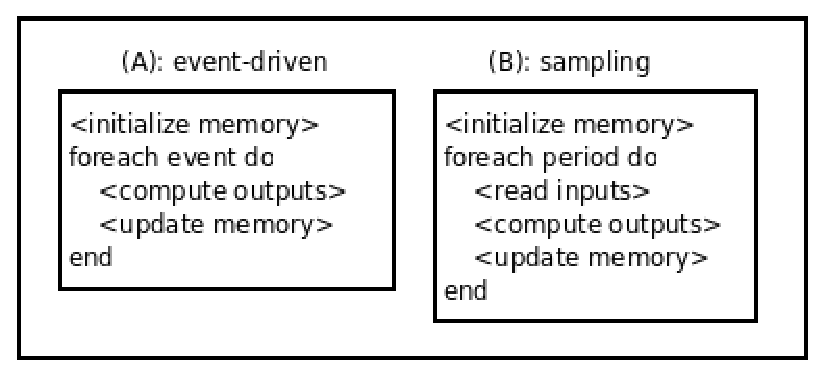
\includegraphics[width=3.0in]{sync_impl.eps}
\caption{Schedulers for synchronous systems}
\label{fig.impl}
\end{figure}
% Esterel, HW, \CEU, observers

Figure \ref{fig.impl} shows two common implementation schemes for synchronous 
schedulers~\cite{rp.twelve}.
%
in the event-driven scheme, a loop iteration computes outputs for each event 
occurrence;
%
in the sampling scheme, a loop iteration computes the inputs and outputs on 
every clock tick.
%
In both cases, each loop iteration represents a logical instant in which the 
system as a whole reacts synchronously before going to the next instant.
%
During a reaction, the environment is invariant and does not affect the running 
iteration%
\footnote{
An actual implementation enqueues incoming input events to process them in the 
next iterations.
}.
%
Both schemes are compliant with the synchronous hypothesis, in which input and 
resulting output happen at the same time, considering this notion of time as a 
sequence of discrete events or clock ticks.
%end{comment}

%begin{comment}
%
Having the language to deal automatically with these features strengthen 
structured programming, because we can compose activities together.
%
For instance, although adding a new activity implies extra computational 
overhead, it does not affect the behavior of the other activities, which still 
depend only on the input timeline.
%
Furthermore, if we want to abort an existing activity given a new requirement, 
we can do it externally, without changing

 determinism and abortion with these issues is interesting allows to
compose activities while keeping them decoupled, because they need not to be 
NOtweaked to accommodate these requirements.


decoupling =>
structured programming

deterministic,
    reproducible
abortion
    structured programming
    no coupling
    just like

The way each side is implemented does not affect the behavior,
only the way you compose them (which is external to each implementation)

%
DET and ABRT
both yield to better reasoning
behave the same with or without concurrency
%end{comment}

%%%%%%%%%%%%%%%%%%%%%%%%%%%%%%%%%%%%%%%%%%%%%%%%%%%%%%%%%%%%%%%%%%%%%%%%%%%%%%%

\subsection{Deterministic execution}

In the context of reactive applications, we interpret determinism as 
reproducible execution given the same sequence of stimuli, i.e., the outcome 
depends exclusively of an external input timeline, in contrast with internal 
scheduling and communication timings.

Figure~\ref{lst.leds} shows three implementations for an application that 
blinks two LEDs in parallel with different frequencies.
We use two asynchronous languages (a CSP-based~\cite{arduino.occam} and a 
thread-based~\cite{arduino.chibios} language), and also the synchronous 
language \CEU.
%
The intent and syntactic structure of the implementations are similar:
composing the two blinking activities in parallel.
%
The LEDs should blink together every 3 seconds (the least common denominator 
between 600ms and 1s).
%
As we expected, the LEDs in the two asynchronous implementations loose 
synchronism after some time of execution, while the implementation in \CEU 
remains synchronized forever.

The example highlights how the inherent non-determinism in the asynchronous 
model makes hard to (blindly) compose activities supposedly synchronized: 
unpredictable scheduling as wall as latency in message-passing eventually cause 
observable asynchronism.
%
In \CEU, the \code{await} is the only primitive that takes time, but which the 
programmer uses explicitly to conform with the problem specification.
The language runtime compensates the internal timings for communication and 
computation (which the programmer cannot control) to conform with the model and 
remain synchronized~\cite{ceu.sensys13}.
%
Arguably, reasoning over \code{await} statements is simpler than also having to 
consider all other statements of the language.

\begin{figure}[t]
\begin{minipage}[t]{0.34\linewidth}
\begin{lstlisting}
// OCCAM-PI
PROC main ()
 CHAN SIGNAL s1,s2:
 PAR
  PAR
   tick(600, s1!)
   toggle(11, s1?)
  PAR
   tick(1000, s2!)
   toggle(12, s2?)
:

\end{lstlisting}
\end{minipage}
%
\begin{minipage}[t]{0.33\linewidth}
\begin{lstlisting}
// ChibiOS
void thread1 () {
  while (1) {
    sleep(600);
    toggle(11);
  }
}
void thread2 () {
  while (1) {
    sleep(1000);
    toggle(12);
  }
}
void setup () {
  create(thread1);
  create(thread2);
}

\end{lstlisting}
\end{minipage}
%
\begin{minipage}[t]{0.31\linewidth}
\begin{lstlisting}
// Ceu
par do
  loop do
    await 600ms;
    _toggle(11);
  end
with
  loop do
    await 1s;
    _toggle(12);
  end
end
\end{lstlisting}
\end{minipage}
%
%\rule{8.5cm}{0.37pt}
\caption{ Two blinking LEDs in OCCAM-PI, ChibiOS and \CEU.\newline
{\small %\textmd{
%The lines of execution in parallel blink two LEDs (connected to ports 11 and 
%12) with different frequencies.
%Every 3 seconds the LEDs should light on together.
}%}
\label{lst.leds}
}
\end{figure}

%%%%%%%%%%%%%%%%%%%%%%%%%%%%%%%%%%%%%%%%%%%%%%%%%%%%%%%%%%%%%%%%%%%%%%%%%%%%%%%

\subsection{Orthogonal abortion}

%begin{comment}

On the other hand, the synchronous hypothesis does not hold for reactions that 
have latency (e.g., network communication or algorithm-intensive computations),
however, does not apply when the computation involves latency:
problem communication takes time
either communication or time consuming operations
because now, at the speed of the program

parallelism
latency

For reactive systems zzz
For highly synchronous systems, the sole synchronization overhead, which is 
non-existent in XXX, may neutralize any gains with parallelism.
% or even worsen parallelism

Illustrate with two examples:
that explore the advantages of synchronous:
reasoning in concurrency
seamless composition

communitacions is directed and takes time (because the receiver may not be 
waiting)

The synchronous model
input => output
broadcast possible
global consensus possible
determinism
simpler model

In synchronous systems, communication is instantaneous.
The zero-delay property of the synchronous hypothesis guarantees that no time 
elapses between event announcement and receiving.
Also, as communication is via broadcast, all systems parts share the same 
information all the time.
These two characteristics make global data consensus another property of 
synchronous systems.

conclusion:
no blind/free/orthogonal composition
no deterministic/reproducible execution
parallelism / no-forced synch
time-consuming / independent

A recent Reactive Manifesto

synchronous reactive
vs
asynchronous reactive

Even tough the presented deterministic and abortion examples can be properly 
implemented in asynchronous languages, they require to tweak the activities 
with mutual
synchronization primitives.
%
This increases the coupling degree among activities with concerns that are not 
directly related to the problem specification.

The two models suggest a tradeoff between unrestricted execution with real 
parallelism versus structural composability with deterministic behavior.
%
For reactive applications with continuous and real-time concurrency, we believe 
that the synchronous execution model is more appropriate.

\end{comment}

\end{document}
